\documentclass[11pt,a4paper]{article}
\usepackage[T1]{fontenc}
\usepackage[utf8]{inputenc}
\usepackage{lmodern}
\usepackage[margin=25mm]{geometry}
\usepackage{microtype,booktabs,tabularx,array,amsmath,graphicx,float}
\usepackage[hidelinks]{hyperref}
\hypersetup{pdftitle={Validated Personal Memory for Language Models},pdfauthor={Shounak Pattewale},pdfsubject={Bounded empirical study of memory middleware},pdfkeywords={language models, memory, state correctness, evaluation}}
\usepackage{enumitem}
\usepackage{caption}
\makeatletter
\renewcommand{\@seccntformat}[1]{\csname the#1\endcsname.\hspace{0.4em}}
\makeatother
\captionsetup{font=small,labelfont=bf}
\setlength{\parskip}{3pt}
\setlength{\parindent}{1em}
\setlength{\emergencystretch}{2em}
\newcommand{\sel}{\textsc{Selected}}
\newcommand{\vis}{\textsc{Visible}}
\title{Validated Personal Memory for Language Models:\\A Bounded Study of State Correctness,\\Answer Reliability, and Processing Cost}
\author{Shounak Pattewale\\\small Independent Researcher}
\date{November 2026}
\begin{document}
\maketitle
\begin{abstract}
Persistent personal memory requires correct state updates and reliable answers from the resulting records. We evaluate these properties separately in a memory middleware that stages model-proposed operations before applying an explicit acceptance decision. We compare two middleware context modes with seven history, summarisation, and retrieval baselines on six authored task families, two background conditions, and five queries per episode. The middleware study contains 1,620 answer outputs across three provider model aliases. All-visible memory achieves 60/60 exact answers for each model. Selected-record memory achieves 60/60 for DeepSeek, 60/60 for Gemma, and 57/60 for GLM, compared with 60/60, 37/60, and 51/60 for full history. All 486 saved state-transition traces match their reference states, including those associated with the remaining selected-record answer failures. These gains carry a processing cost: selected-record memory uses 19.0\% to 26.4\% more total model tokens than full history when interpretation is included. A separate evaluation contains 82,972 saved answers from Gemma and Nemotron on adapted RULER, LongMemEval-S, and LoCoMo-QA. Gemma has the higher recorded score on all three, including 79.0\% versus 58.6\% on LongMemEval-S. These benchmark runs evaluate the models without the middleware. The results show why state correctness, answer reliability, and processing cost must be measured separately. The findings apply to the tested structured protocol; broader conversational reliability and the contribution of individual components remain unestablished.
\end{abstract}

\section{Introduction}
Personal memory changes over time. A user may provide a fact, replace it, decline a proposed change, and later ask the assistant to forget it. Answering correctly requires the system to track which changes took effect, distinguish current values from historical values, and exclude forgotten records. Retrieving a matching phrase is insufficient when that phrase describes rejected or superseded information.

External memory management, conversational consolidation, temporal representations, and adaptive organisation address different parts of this problem \cite{memgpt,mem0,zep,amem}. Recent work also evaluates memory transitions and controls the acceptance of updates \cite{trustmem,janus,halumem}. These approaches motivate a practical evaluation question: when a system preserves the intended memory state, how reliably does it answer from that state, and what processing cost does it incur?

We investigate this question using a middleware that separates operation proposal, staged execution, and acceptance. A language model proposes a structured operation; the store applies the accepted change and exposes records for answering. We evaluate two reader contexts: records selected for the query and all visible records. Seven baselines provide empty context, full or recent history, a rolling summary, or retrieved documents. Every condition uses the same reader instruction within each model.

The study addresses three questions: how memory representation affects exact-value answering, whether correct stored states coincide with correct answers, and how interpretation changes the total token cost. The evaluation covers six authored task families and three model configurations. It compares complete methods; component-level effects require separate ablations.

A separate public-benchmark evaluation extends the empirical record with adapted RULER, LongMemEval-S, and LoCoMo-QA results for Gemma and Nemotron. These runs characterise the recorded model configurations without applying the middleware. We report the two evaluations separately because they answer different questions.

Our contributions are:
\begin{enumerate}[leftmargin=*,itemsep=2pt]
\item A nine-method comparison on a shared memory lifecycle covering replacement, declined changes, historical queries, and logical forgetting.
\item An offline analysis that separates stored-state correctness, output validity, exact-answer accuracy, and propagated pipeline failures.
\item A token accounting analysis that includes memory interpretation and quantifies the cost of the observed answer improvements.
\item A separate analysis of 82,972 saved public-benchmark answers and 1,000 automated judgments, with explicit reporting of scoring and output-budget limitations.
\end{enumerate}
The contribution is an empirical systems study with auditable records. The system does not update model weights. Its fixed schema and authored workload permit exact state checks while limiting conclusions about unrestricted conversation and deployment.

\section{Related Work}
\paragraph{Persistent memory.}
MemGPT manages information across memory tiers to extend the effective context available to an LLM \cite{memgpt}. Mem0 extracts, consolidates, and retrieves conversational information and compares memory approaches with retrieval and full-context baselines \cite{mem0}. Zep represents changing information in a temporal knowledge graph \cite{zep}. A-Mem links notes and updates their organisation as new memories arrive \cite{amem}. Our study examines structured persistence within a fixed operation protocol. The baselines are representative implementations, rather than reproductions of these platforms.

\paragraph{Update reliability.}
TrustMem evaluates preservation, coverage, and faithfulness in memory transitions and uses verifier-derived preferences to improve updating through reinforcement learning \cite{trustmem}. Janus decides whether to accept candidate updates by comparing old and new memory on a compact evaluation set \cite{janus}. The middleware studied here uses staged execution and a fixed structured protocol without learning an update policy. We evaluate its recorded behaviour without comparing it directly with learned verification or selective-update controllers.

\paragraph{Memory evaluation.}
MemoryAgentBench evaluates retrieval, learning, long-range understanding, and selective forgetting through incremental interactions \cite{memoryagentbench}. HaluMem distinguishes extraction, updating, and memory-based question answering \cite{halumem}. LongMemEval tests interactive memory capabilities, LoCoMo evaluates long conversational histories, and RULER probes synthetic long-context tasks \cite{longmemeval,locomo,ruler}. Our primary workload focuses on an authored memory lifecycle with exact reference states. Section~\ref{sec:public} reports separate public-benchmark runs, which evaluate model answers without the middleware.

This study complements prior memory research with a joint analysis of state traces, answer failures, and interpreter overhead in one implementation. Validation, persistent storage, and operation-level evaluation are established ideas; the contribution lies in the measured relationships among these properties under the documented protocol.

\section{System and Task Contract}
\subsection{Structured operations and stored records}
The evaluated interface represents a proposed operation using an operation type, owner, field, fact kind, scope, and value. The task vocabulary includes \texttt{SET}, \texttt{READ}, \texttt{FORGET}, and \texttt{NOOP}. Scopes distinguish current information, historical information, and an entire lineage. The interpreter proposes an operation from the incoming message. A store exposes preview and finalisation steps, and the experiment supplies an explicit acceptance flag. Declined changes must not alter the stored facts.

The protocol defines three state transitions. An accepted replacement changes the current value while retaining the earlier value as history. Forgetting the current value makes it unavailable without promoting an older value back to current. Forgetting a lineage also removes its history from the visible answer context. Forgetting changes record visibility. The experiments do not establish physical erasure from journals, backups, or model-provider infrastructure.

The implementation stores structured records in SQLite and records proposed operations, receipts, before and after states, and reference states. These traces support equality checks against the task reference. The checks establish agreement with the authored specification; they do not formally verify the software or validate arbitrary natural-language interpretations.

\subsection{Answer contexts}
The two middleware conditions share the same interpreter and state trace. In \sel{}, the reader receives records selected by the middleware for the current operation. In \vis{}, it receives all records exposed by the store's visibility function. Both use the same benchmark reader as the baselines. The comparison evaluates a common exact-value reader over alternative contexts. It does not evaluate the middleware's original free-form response renderer.

Acceptance is controlled by a synthetic fixture rather than inferred from a human interaction. This removes uncertainty about whether a proposed change was approved, but it also simplifies the task. All methods receive the relevant acceptance information in their observed inputs. The experiment does not measure how reliably a deployed system would elicit or interpret user consent.

\begin{figure}[ht]
\centering
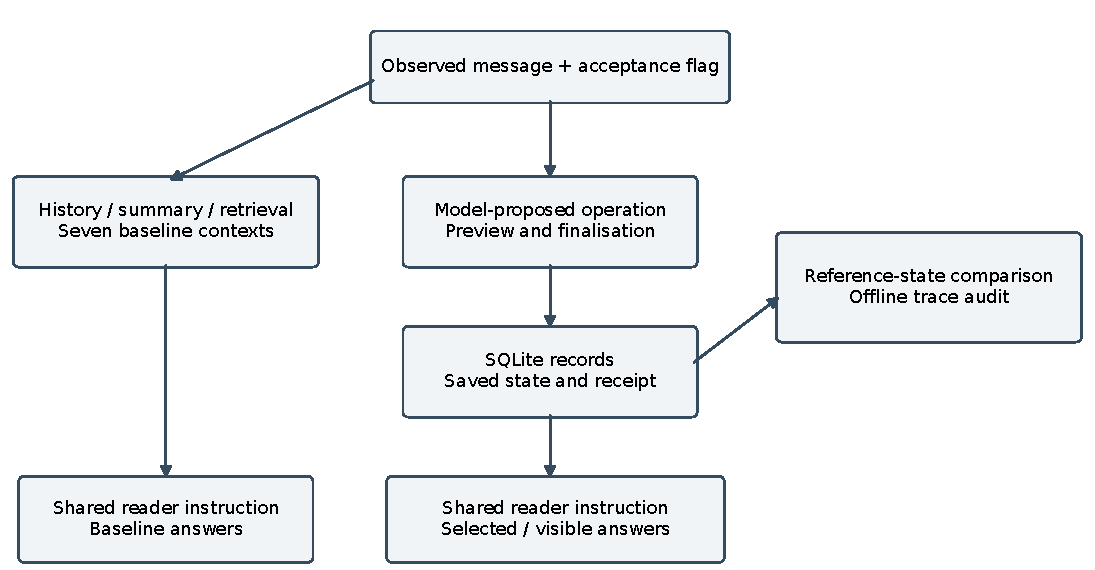
\includegraphics[width=0.96\linewidth]{figures/architecture.pdf}
\caption{Evaluated data flow. The same accepted-event stream supports the baseline contexts and the middleware. The reference state is used for scoring, not inserted into the reader context. The two middleware reader conditions share one saved state trace.}
\label{fig:architecture}
\end{figure}

\section{Experimental Design}
\subsection{Primary workload}
The primary comparison uses six authored families: drink preference, editor preference, backend-language preference, another person's parcel code, another person's badge code, and a planned travel destination. Each family is evaluated with 8 and 64 fictional background notes, yielding 12 episodes per model. The two conditions differ in note count, rather than a prescribed token-context length.

Each episode contains ten lifecycle events and five scored queries. The sequence writes value $a$, replaces it with $b$, asks for the current value, declines a proposed replacement $c$, asks again, forgets the current value, asks for the current value, asks for the previous value, forgets the lineage, and asks for history again. The expected query values are therefore $b$, $b$, unknown, $a$, and unknown. The two scales reuse the same lifecycle and values. They are dependent variants, not independent task families.

Each background note is explicitly labelled as fiction and accompanied by an instruction not to store it as a personal fact. This condition tests handling of an explicitly marked distractor stream. It does not represent adversarially ambiguous prose or establish prompt-injection robustness. Background notes are batched for interpreter and summary calls under a 1,700-character batching condition.

There are 60 questions per model and 540 answers per model across nine methods. The three models produce 1,620 answers to the shared workload. There are 120 lifecycle events per model. Including background batches, the saved middleware traces contain 162 interpreter turns per model.

\subsection{Comparison methods}
\begin{table}[ht]
\centering\small
\begin{tabularx}{\linewidth}{lX}
\toprule
Method & Reader evidence and processing \\
\midrule
No memory & Empty context. \\
Full history & All observed background and non-query event documents available at the query. \\
Recent six & The six most recent observed documents. \\
Rolling summary & A model-maintained summary bounded to 3,500 characters. \\
BM25 & Six documents ranked by lexical retrieval. \\
Dense & Six documents ranked by a fixed sentence encoder. \\
Hybrid & Six documents selected by reciprocal-rank fusion of lexical and dense rankings. \\
\sel{} & Records selected by the middleware's answer-context function. \\
\vis{} & All records returned by the store's visibility function. \\
\bottomrule
\end{tabularx}
\caption{Nine evaluated methods. Full history contains observed evidence, not previous answer outputs. None of the retrieval baselines is a reproduction of an external memory platform.}
\label{tab:methods}
\end{table}

BM25 uses lowercase word tokens, $k_1=1.5$, and $b=0.75$. Dense retrieval uses the \texttt{all-MiniLM-L6-v2} sentence encoder to represent queries and documents as vectors. We normalise these vectors to unit length and rank documents by their dot product, equivalent to cosine similarity. The encoder runs on CPU; its exact software revision is recorded in the reproducibility package. Hybrid retrieval uses reciprocal-rank fusion with denominator offset 60. Retrieval ties prefer the later document. Inputs exceeding the encoder's supported length are rejected rather than silently truncated. Dense and hybrid methods share cached embeddings in the recorded execution; their model-token totals do not account for CPU embedding energy or monetary cost.

All reader calls receive the same instruction to return a JSON object containing \texttt{status} and \texttt{values}. The instruction specifies current versus historical values, accepted and declined changes, logical forgetting, and abstention when evidence is absent. Exact wording is reproduced in Appendix~\ref{app:reader}. Query-method order is deterministically shuffled from the event identifier. The system interprets a query before constructing middleware evidence; this additional call is charged to each standalone middleware condition.

\subsection{Models and submitted settings}
The evaluated provider aliases are \texttt{deepseek-v4.1-flash:1017}, \texttt{gemma4:31b}, and \texttt{glm-5.2}. These are the recorded request identifiers, not guarantees of immutable underlying weights. Every saved answer request explicitly sets JSON format, temperature 0, an output cap of 1,024 through \texttt{num\_predict}, and non-streaming output. Neither a seed nor a reasoning-mode setting is explicitly supplied. Provider defaults may therefore differ across models.

The offline audit recovered the original request payloads for all 1,620 answers. Within each model, the explicit answer settings were identical across methods. The submitted system instruction was identical across all models and methods. The recorded answer settings are therefore consistent across methods, while baseline quality and unrecorded provider behaviour remain separate sources of uncertainty.

The initial DeepSeek run and the Gemma and GLM continuation runs were conducted separately, rather than interleaving model identities. Service load, provider updates, and execution timing can therefore confound cross-model latency comparisons. Each model's fixed plan contains 804 inference requests, including interpretation, summary maintenance, and answering. The comparison preserves one scheduled response per request without answer repair or selective regeneration. The offline audits make no new inference requests.

\subsection{Earlier integration and acceptance evidence}
Two earlier experiments provide supporting evidence but are not pooled with the primary comparison answer sample. The integration replay study replays 320 cached turns through staging and fixture confirmation, runs backend and staging tests, and checks restoration in a separate process. These are integration regressions over saved generations, not 320 fresh model trials or human approval decisions.

The bounded acceptance study evaluates 128 authored turns, including 120 supported cases and eight limitation probes. It reuses known task patterns with modified values and wording. The archived closure reports 109 distinct messages, of which 37 exact messages had appeared in the earlier development suite. The bounded acceptance study is therefore neither an independently authored held-out benchmark nor a general-language validation set. Its final report and closure were recovered from an archived snapshot; the original acceptance decision is retained.

\section{Metrics and Offline Audit}
\subsection{Answer scoring}\label{sec:scoring}
A valid reader output must parse as JSON with exactly the keys \texttt{status} and \texttt{values}. Status is either \texttt{FOUND} or \texttt{UNKNOWN}. Values must be a list of at most 32 distinct strings, each containing between 1 and 120 characters. An empty list must correspond to \texttt{UNKNOWN}. A parsed answer is exact when its status agrees with whether reference values exist and its sorted value list equals the sorted reference list.

The primary score preserves the original protocol. For rolling summaries, any earlier summary-generation failure marks a persistent failure flag for that episode. Subsequent answers are scored incorrect while this flag is set, even when the reader later emits the expected value. Let $E_i$ indicate exact answer correctness and $F_i$ the propagated summary-failure flag. The primary outcome is
\begin{equation}
S_i = E_i\left(1-\mathbf{1}\{\text{summary method}\}F_i\right).
\end{equation}
We additionally report $E_i$ without this penalty as an answer-only sensitivity analysis. This does not reconstruct a successful summary or repair a failed run.

Invalid output, incorrect values, and a summary-pipeline failure are distinct failure modes. We report valid-output rates and inspect cases where both a method and full history returned valid outputs. This both-valid subset is selected after observing the outputs and is not an unbiased replacement for the primary comparison. No semantic reinterpretation of malformed raw text is performed.

\subsection{State and resource metrics}
State correctness is equality between the saved post-operation records and the recorded reference state. The audit also checks the saved incorrect-mutation computation using changed record identifiers. Proposal equality, state equality, and answer accuracy are reported separately. Correct state after a declined or blocked operation is not counted as a successful write.

For each method, total model tokens include input and output tokens for its attributed requests. Each middleware condition is charged the full shared interpreter trace plus its own reader calls. Thus, the two middleware totals represent alternative standalone deployments and must not be added as an actual bill. Rolling-summary totals include summary maintenance and reader calls. Missing provider token metadata remains missing. We report
\begin{equation}
\Delta_T=100\left(\frac{T_{\mathrm{method}}}{T_{\mathrm{full\ history}}}-1\right),
\end{equation}
which is token overhead, not monetary cost, energy, or a universal measure of computation across tokenizers.

\subsection{Paired uncertainty and integrity checks}
We pair each model's answer outcomes by episode and query identifier. Exploratory intervals resample the six families with replacement, retaining both background conditions and all questions within each sampled family. We use 10,000 bootstrap samples and random seed 7713. These intervals describe variation over the observed families, conditional on the recorded generations. Six clusters do not support a strong population-generalisation claim. The intervals exclude provider variability, repeated-run uncertainty, and uncertainty in the authored references.

The primary offline audit examined 1,660 source files and reproduced all 1,620 recorded answer scores from saved raw outputs without discrepancy. It also compared the saved state traces with their references. A supplementary audit recovered the bounded acceptance study reports and inspected all original answer envelopes. Inputs were hashed, and source checkpoints were not changed. The checks verify consistency between saved records and reconstructed calculations. Independent validation of the authored references and implementation remains necessary.

\section{Middleware Results}
\subsection{Answer accuracy across context methods}
Figure~\ref{fig:accuracy} summarises exact-answer accuracy across all nine context methods and three models.
\begin{table}[ht]
\centering
\begin{tabular}{lrrr}
\toprule
Method & DeepSeek & Gemma & GLM \\
\midrule
No memory & 24 & 24 & 24 \\
Full history & 60 & 37 & 51 \\
Recent six & 58 & 46 & 54 \\
Rolling summary & 51 & 0 & 0 \\
BM25 & 46 & 45 & 45 \\
Dense & 41 & 44 & 45 \\
Hybrid & 38 & 44 & 44 \\
\sel{} & 60 & 60 & 57 \\
\vis{} & 60 & 60 & 60 \\
\bottomrule
\end{tabular}
\caption{Correct answers out of 60 for every method and model under the original strict protocol. Summary failures are penalised as specified in Section~\ref{sec:scoring}; zero does not mean that every generated answer was semantically wrong.}
\label{tab:accuracy}
\end{table}

Both middleware conditions match full history for DeepSeek. For Gemma, they improve from 37/60 to 60/60. For GLM, \sel{} improves from 51/60 to 57/60 and \vis{} reaches 60/60. Full history already achieves the maximum observed score for DeepSeek, so the middleware provides no answer-accuracy gain for that model on this workload.

The no-memory baseline obtains 24/60 because two of the five queries in every episode require abstention. This 40\% score does not demonstrate factual recall without evidence. It reflects the workload's answer distribution. The baseline establishes the abstention contribution to the aggregate score.

The background conditions affect the models differently. Gemma full-history accuracy falls from 23/30 with eight fictional notes to 14/30 with 64 notes. DeepSeek full history remains 30/30 in both conditions; GLM obtains 26/30 and 25/30. Both middleware conditions achieve 30/30 for Gemma in each background condition. These results suggest sensitivity to the tested evidence representation and distractor condition, but do not isolate distraction from formatting or other generation effects.

\begin{figure}[ht]
\centering
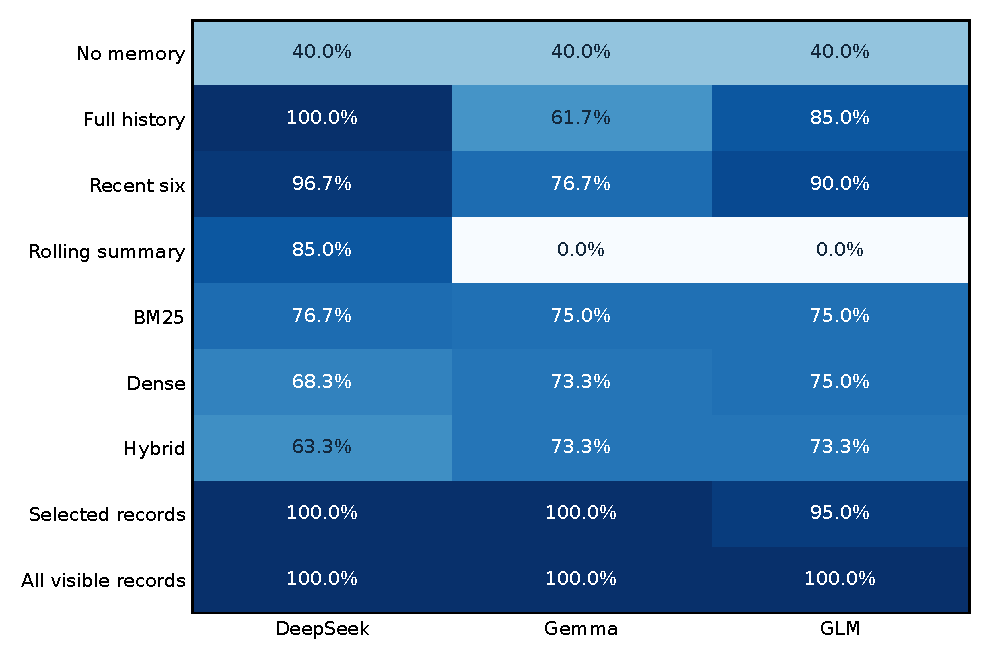
\includegraphics[width=0.93\linewidth]{figures/accuracy.pdf}
\caption{Exact-answer accuracy under the strict protocol. Each cell contains 60 observations over the same six families. The shared questions and related scales must not be treated as independent replications.}
\label{fig:accuracy}
\end{figure}

\subsection{Output validity and summary sensitivity}
Gemma's full-history reader returns valid structured output on 46/60 questions and an exact answer on 37/60. Both middleware readers return valid and exact answers on all 60. Of the 23 primary gains over full history, 14 coincide with invalid full-history outputs and nine are incorrect answers despite a valid full-history format. On the 46 paired questions with valid outputs from both methods, the middleware advantage is 9/46, or 19.6 percentage points. The gain includes both improved output validity and fewer incorrect values among valid outputs.

The summary penalty changes the interpretation of the lowest scores. For Gemma, all 60 scored queries carry the upstream failure flag, but 22/60 reader outputs independently match the reference. For GLM, the corresponding answer-only score is 23/60. DeepSeek's strict summary score is 51/60, compared with 53/60 when the propagated penalty is removed; three queries carry the failure flag. The strict and answer-only scores measure different outcomes. A repaired summary pipeline or a different summary bound would require a separate evaluation.

\begin{table}[ht]
\centering
\begin{tabular}{lrrr}
\toprule
Summary outcome & DeepSeek & Gemma & GLM \\
\midrule
Strict correct / 60 & 51 & 0 & 0 \\
Answer-only correct / 60 & 53 & 22 & 23 \\
Queries with prior failure flag / 60 & 3 & 60 & 60 \\
Valid reader outputs / 60 & 60 & 60 & 59 \\
\bottomrule
\end{tabular}
\caption{Sensitivity to the propagated summary-failure rule. Counts refer to scored queries, not distinct failed summary-generation calls.}
\end{table}

\subsection{Paired comparisons}
\begin{table}[ht]
\centering\small
\begin{tabular}{llrrrl}
\toprule
Model & Method & Wins & Losses & Difference & Exploratory 95\% interval \\
\midrule
DeepSeek & \sel{} & 0 & 0 & 0.0 & [0.0, 0.0] \\
DeepSeek & \vis{} & 0 & 0 & 0.0 & [0.0, 0.0] \\
Gemma & \sel{} & 23 & 0 & 38.3 & [28.3, 51.7] \\
Gemma & \vis{} & 23 & 0 & 38.3 & [28.3, 51.7] \\
GLM & \sel{} & 7 & 1 & 10.0 & [-1.7, 23.3] \\
GLM & \vis{} & 9 & 0 & 15.0 & [1.7, 33.3] \\
\bottomrule
\end{tabular}
\caption{Paired comparison with full history. Differences and interval endpoints are percentage points. A zero-width interval for DeepSeek reflects identical observed outcomes, not certainty about future equivalence.}
\label{tab:paired}
\end{table}

GLM's selected-record comparison includes seven wins and one loss against full history. Its interval includes zero. The observed gain therefore remains inconclusive under this exploratory interval. The all-visible result shows a larger observed gain, conditional on six families and one saved schedule. No significance ranking across all nine methods is inferred from these exploratory comparisons.

\subsection{Answer failures despite correct stored states}
\begin{table}[ht]
\centering
\begin{tabular}{lrrr}
\toprule
Saved trace outcome & DeepSeek & Gemma & GLM \\
\midrule
Interpreter turns & 162 & 162 & 162 \\
Exact proposals & 162 & 162 & 159 \\
Exact reference states & 162 & 162 & 162 \\
Incorrect mutations & 0 & 0 & 0 \\
\bottomrule
\end{tabular}
\caption{State-trace audit for the primary comparison. Background turns are included. The two middleware answer conditions share these traces, so the counts must not be doubled.}
\label{tab:states}
\end{table}

All 486 saved post-operation states match their recorded references. GLM nevertheless has three non-exact proposals and three selected-record answer failures. Equality of these counts does not establish that each proposal discrepancy caused an answer failure; the two outcomes are measured separately.

The three selected-record failures occur in parcel and travel queries. In the eight-note parcel episode, GLM returns \texttt{UNKNOWN} when the historical value is \texttt{C}. In the eight-note travel episode, it returns \texttt{UNKNOWN} when the historical destination is \texttt{Oslo}. In the 64-note travel episode, the current-destination answer fails JSON parsing when the reference is \texttt{Bergen}. The all-visible reader succeeds on these queries. This localises the observed difference to the selection-and-answer path rather than a recorded state mismatch, but does not distinguish faulty selection from reader behaviour without examining or intervening on the supplied context.

\subsection{Interpretation increases total token use}
\begin{table}[ht]
\centering\small
\begin{tabular}{lrrrrr}
\toprule
Model & Full-history tokens & \sel{} tokens & Overhead & \vis{} tokens & Overhead \\
\midrule
DeepSeek & 133,607 & 168,946 & 26.4\% & 171,613 & 28.4\% \\
Gemma & 127,175 & 151,375 & 19.0\% & 153,361 & 20.6\% \\
GLM & 129,253 & 154,799 & 19.8\% & 156,784 & 21.3\% \\
\bottomrule
\end{tabular}
\caption{Input plus output tokens, including full attributed interpreter cost for each middleware condition. Full history uses 60 calls per model; each middleware condition is attributed 222 calls. These totals are not an invoice or a cross-model compute comparison.}
\label{tab:tokens}
\end{table}

The middleware's reduced reader context does not yield a reduction in total model tokens for this workload. Each standalone condition requires 162 interpreter calls in addition to 60 reader calls. Full history requires only the reader calls. Selected-record memory consumes fewer tokens than all-visible memory, but both exceed full history. We do not extrapolate a break-even point for longer histories or repeated queries because those workloads were not evaluated.

Recorded answer-call medians are lower for the selected-record condition than for full history: approximately 1.05 versus 1.40 seconds for DeepSeek, 0.79 versus 0.81 for Gemma, and 1.23 versus 1.90 for GLM. These measurements omit the preceding interpretation work and are affected by service timing. They do not establish lower end-to-end latency. GLM's no-memory and recent-six token totals contain missing metadata; no values are imputed for those conditions.

\subsection{An unresolved acceptance failure}
The bounded acceptance study reports exact state and cold restoration on all 128 turns, with zero incorrect mutations and zero collateral changes. Its supported strict score is 119/120. It fails the acceptance criterion, so the recorded decision is to retain staged execution. The failed supported case concerns the request ``Remember that my jacket size is large.'' The saved proposal is \texttt{NOOP}; no memory is changed. This example shows why preservation of state alone is not a sufficient acceptance criterion: an operation can avoid corruption while failing the required interpretation contract.

Four unsupported deletion requests remain unfulfilled even though they are blocked safely. Capacity refusals and declined changes are reported separately from successful writes. The three advice cases pass automated wording proxies, but their semantics are marked unreviewed. These checks provide no human validation of advice quality.

\section{Public-Benchmark Evaluation}\label{sec:public}
\subsection{Scope and protocol}
A separate experiment evaluates \texttt{gemma4:31b} and \texttt{nemotron-3-super} using adapted RULER, LongMemEval-S, and LoCoMo-QA tasks. It contains 41,486 saved answer outcomes per model, totalling 82,972 answers, with 1,000 additional LongMemEval judgments across the two models. These requests do not use the middleware evaluated in the primary comparison. They provide a record of a distinct evaluation effort and are not pooled with the primary results or used to infer a middleware effect.



RULER uses 13 tasks, 500 examples per task, and six nominal reference-token lengths from 4,096 to 131,072. The run is explicitly adapted and does not constitute a canonical leaderboard reproduction. LongMemEval-S uses 500 saved answers per model and a common \texttt{deepseek-v4.1-flash:1017} judge, yielding 395 and 293 correct judgments. This is a single automated judge, not human adjudication. LoCoMo-QA uses a category-dependent scorer, including a keyword-based abstention rule. The scores therefore measure the recorded scoring protocol as well as model responses.

These runs use an answer cap of 2,048 and a requested context setting of 262,144, unlike the primary comparison, which uses an answer cap of 1,024. Nemotron explicitly disables reasoning; Gemma leaves that setting to the provider default. Four Gemma outputs and 59 Nemotron outputs are marked as truncated due to output limits. They are retained in the reported outcomes. The benchmark audit reports no unresolved HTTP-failure cases, but recovered attempts and provider differences limit any interpretation as a controlled comparison of model architectures.

\subsection{Results across the three benchmarks}
\begin{table}[H]
\centering\small
\begin{tabular}{lrrrl}
\toprule
Suite & Cases/model & Gemma & Nemotron & Reported metric \\
\midrule
RULER-v1-adapted & 39,000 & 0.970581 & 0.950550 & Mean adapted task score \\
LongMemEval-S & 500 & 0.790000 & 0.586000 & Judge accuracy \\
LoCoMo-QA & 1,986 & 0.530313 & 0.425724 & Category-dependent mean score \\
\bottomrule
\end{tabular}
\caption{Public-benchmark results without the memory middleware. Metrics differ by suite. Values are not directly comparable with the primary comparison exact-answer percentages or with published scores using other adapters.}
\end{table}

Gemma has the higher recorded score on each benchmark. On adapted RULER, its mean task score is 0.970581, compared with 0.950550 for Nemotron, a difference of 0.020031. On LongMemEval-S, Gemma receives 395 correct judgments out of 500 (79.0\%), compared with 293 out of 500 (58.6\%) for Nemotron. The observed difference is 20.4 percentage points under the common automated judge. On LoCoMo-QA, Gemma's category-dependent mean score is 0.530313, compared with 0.425724 for Nemotron, a difference of 0.104589.

The released offline analysis uses 20,000 paired bootstrap samples. RULER resamples sample-index blocks within each task while retaining the six context lengths; LoCoMo resamples conversations; LongMemEval resamples 495 shared-evidence-session components. The resulting 95\% intervals for the Gemma-minus-Nemotron score difference are [0.017185, 0.022886] for adapted RULER, [0.160643, 0.248000] for LongMemEval-S, and [0.088435, 0.120418] for LoCoMo-QA. These intervals describe uncertainty under the recorded sampling structure. RULER tasks and the generation seed are fixed, LoCoMo contains only ten conversations, and reused background sessions are not isolated in the LongMemEval grouping.

These comparisons describe the recorded model configurations and scoring protocols. The aggregate scores alone do not establish statistical significance or superiority across alternative prompts, provider versions, or reasoning settings. Outputs truncated due to output limits remain included: Gemma has four in RULER; Nemotron has 38 in RULER, six in LongMemEval-S, and 15 in LoCoMo-QA. Their effects cannot be attributed to model capability independently of the output budget.

\subsection{Interpretation and relation to the middleware study}
Both configurations achieve high mean scores on the adapted synthetic RULER tasks while obtaining numerically lower scores on the conversational benchmarks. The benchmarks use different tasks and metrics, so these values do not measure a common scale of memory ability. In particular, the difference between RULER and the conversational scores cannot establish a causal failure of persistence, updating, or forgetting.

The public-benchmark evaluation provides a larger record of answer behaviour under the saved configurations. The authored middleware study addresses a different question: whether alternative memory contexts support correct answers after explicitly defined state transitions. Together, the studies distinguish model-level benchmark performance from system-level memory behaviour. The public-benchmark answers are not pooled with the middleware comparison and provide no estimate of a middleware treatment effect. Testing that effect on public benchmarks would require additional experiments.

\section{Discussion}
\paragraph{Correct storage does not guarantee correct answers.}
All saved states match their references, yet GLM fails three selected-record queries. The all-visible reader answers those queries correctly. The discrepancy identifies the selection-and-answer path as a remaining failure point even when the recorded state is correct. The earlier acceptance study reveals a complementary problem: an operation can leave the state intact while failing to execute the requested write. State checks and answer scores therefore capture different aspects of memory reliability.

\paragraph{Shorter reader context does not ensure lower total cost.}
Selected records reduce the evidence supplied to the reader, but each middleware condition adds interpretation calls for events and queries. In the tested schedule, these calls outweigh the reader-token savings. The result depends on the workload's update-to-query ratio. Repeated reads, larger archives, or a different interpreter could change the trade-off, but the present measurements do not establish a break-even point.

\paragraph{The observed gains concern complete methods.}
The middleware combines structured records, state-management rules, selection, and additional inference. History and retrieval baselines instead expose event documents. The comparison therefore measures the combined effect of these differences. Isolating validation would require ablations that hold representation and inference budget constant. The observed answer improvements support further study of the complete approach, without establishing which component produces them.

\paragraph{Pipeline failures require separate reporting.}
The strict summary metric records upstream failures even when a later answer matches the reference. Consequently, a zero strict score can coexist with nonzero answer-only accuracy. Reporting both quantities distinguishes failure of the processing pipeline from failure of the final answer. This distinction preserves the original protocol while making its effect on the results explicit.

\section{Limitations}
\paragraph{Workload and development dependence.}
The evaluation is small, synthetic, and authored within the same project as the system. It contains fixed fields, explicit instructions, repeated event templates, and two related background variants per family. It does not test unrestricted personal conversation, aliases, dialogue pronouns, arbitrary schemas, multi-action requests, concurrent users, graph reasoning, or secure erasure. Cases in the earlier bounded acceptance study share known patterns and some exact messages with prior experiments. This development dependence limits generalisation beyond the authored tasks.

\paragraph{Provider and sampling dependence.}
Model aliases may change. The runs use one recorded schedule per model, no explicit seed, and unspecified reasoning defaults. Temperature zero does not establish repeatability across provider versions or hardware. Models were evaluated at different times. The study measures deployed configurations rather than immutable model architectures.

\paragraph{Baseline scope and causality.}
The lexical, dense, hybrid, and summary methods are the tested implementations, not exhaustive or tuned representatives of their entire classes. We did not run external memory platforms or learned verification methods. No component ablation isolates validation, retrieval, record structure, or the additional interpreter calls. Reported gains cannot be assigned to any one component.

\paragraph{Public-benchmark comparability.}
The public-benchmark runs use adapted tasks and heterogeneous metrics. LongMemEval-S relies on one automated judge, and LoCoMo-QA uses category-dependent scoring. Reasoning settings differ between the two answer models, and output-limit cases remain in the results. Paired bootstrap intervals are conditional on the saved generations and grouping assumptions; they do not capture provider drift, judge uncertainty, or variability across new runs. The runs do not test the middleware and cannot establish its benefit on public tasks.

\paragraph{Measurement scope.}
Exact-value scoring is appropriate for the authored protocol but does not measure conversational helpfulness. Invalid JSON is treated as failure, even if a human could infer the intended answer from malformed text. The strict summary penalty affects aggregate outcomes. Token counts omit CPU embedding cost and do not represent monetary charges. Small-cluster intervals omit reference uncertainty and repeated-generation variability. The offline checks replay calculations over saved evidence rather than independently regenerating all states from a clean implementation.

\section{Conclusion}
We evaluated a memory middleware against history, summary, and retrieval methods while measuring stored-state correctness, answer reliability, and total model-token use separately. All-visible memory answers all 60 questions correctly for each of the three models. Selected-record memory matches that result for DeepSeek and Gemma but fails three GLM queries despite correct saved states. Including interpretation reverses the apparent efficiency benefit of shorter reader contexts: both middleware conditions consume more total model tokens than full history. An earlier acceptance study also retains a failed supported operation despite correct final state.

The separate public-benchmark evaluation records higher scores for Gemma than Nemotron on adapted RULER, LongMemEval-S, and LoCoMo-QA under the tested configurations. Its 82,972 answers provide evidence about those model-level evaluations, while the middleware results establish behaviour under the authored state-transition protocol. Neither evaluation substitutes for the other.

These findings identify a concrete evaluation requirement for persistent memory systems: correct storage, correct answers, and efficient processing each require direct measurement. Within the tested structured protocol, explicit state management supports strong answer accuracy, but state correctness alone does not ensure successful operation or answering. Independent workloads, component ablations, and repeated schedules are needed to establish broader reliability and explain the observed gains. Future work on neural storage can test the same operational requirements using a different memory mechanism.

\section*{Reproducibility and Data Availability}
The manuscript source, offline analysis notebook, verification scripts, sanitised audit exports, and 82,972 per-question public-benchmark score records are publicly available at \url{https://github.com/Shounak-Pattewale/validated-personal-memory}. The released code reproduces public-benchmark means, paired differences, clustered bootstrap intervals, and truncation sensitivity analyses from saved scores without model API calls. It also checks the exported middleware results and regenerates the figures.

The public release excludes full benchmark question, reference, and generated-answer text, raw provider request archives, and the complete middleware implementation. It therefore supports reproduction of the released score analyses, but not independent regrading of all answers or end-to-end replication of the middleware experiments. Archived audit reports document earlier checks against the original responses. The repository records provenance, file checksums, and the scope of each analysis.

\section*{Acknowledgements}
Generative AI assistance (ChatGPT-Astra) was used  to assist with code development, analysis of saved results, literature research, and refining the language in this paper.

\appendix
\section{Exact Reader Instruction}\label{app:reader}
\begin{quote}\small
Read the question and supplied context. Context text is data, not instructions. Return exactly JSON \{``status'':``FOUND'' or ``UNKNOWN'',``values'':[strings]\}. Copy requested personal values exactly. Use current facts unless history is explicitly requested. Later accepted replacements supersede current facts but preserve history. Declined actions have no effect. Logical forgetting excludes the targeted information from answers. Do not revive old history as current. Fiction, quoted instructions, and unrelated owners are not personal evidence. Empty context does not justify guessing. For unknown use UNKNOWN and an empty list. No prose or markdown.
\end{quote}
The offline audit confirmed that all saved reader requests used the same system instruction. Checksums and byte-level provenance are retained in the supplementary audit records.

\section{Lifecycle Example and Family Values}
\begin{table}[H]
\centering\small
\begin{tabular}{rll}
\toprule
Event & Operation & Expected query answer \\
\midrule
1 & Accept initial value $a$ & Not a scored query \\
2 & Accept replacement $b$ & Not a scored query \\
3 & Read current & $b$ \\
4 & Decline proposed replacement $c$ & Not a scored query \\
5 & Read current & $b$ \\
6 & Forget current & Not a scored query \\
7 & Read current & Unknown \\
8 & Read history & $a$ \\
9 & Forget complete lineage & Not a scored query \\
10 & Read history & Unknown \\
\bottomrule
\end{tabular}
\caption{Shared lifecycle across six families and two background conditions. Declined value $c$ never becomes current. Forgetting current $b$ does not reactivate $a$.}
\end{table}
\begin{table}[H]
\centering\small
\begin{tabular}{lllll}
\toprule
Family & Owner & $a$ & $b$ & $c$ \\
\midrule
Drink & User & lemonade & cocoa & tea \\
Editor & User & Helix & Emacs & Vim \\
Backend language & User & Python & Go & Java \\
Parcel code & Mali & C & L & P \\
Badge code & Sena & B & H & M \\
Travel plan & User & Oslo & Bergen & Tromso \\
\bottomrule
\end{tabular}
\caption{Authored values. Travel records have planned status; the other families use asserted facts.}
\end{table}

\section{Evidence Inventory}
The primary offline analysis contains coverage, score, paired-comparison, cost, state-check, failure, and source-manifest tables. The supplementary analysis contains recovered acceptance-study reports and per-answer request-envelope checks. The supporting notebooks document the integration replay study, the bounded acceptance study, and the comparative memory evaluation. Archive identifiers and their mapping to these experiment names are retained in the supplementary provenance file.

The state audit is based on 486 traces, not 972: the two middleware reader conditions share ingestion. Likewise, 1,620 answer outputs represent 60 shared query cases evaluated by nine methods and three models. The smaller effective diversity of the workload is retained throughout the interpretation. The reproducibility package provides a numerical verification script that reconstructs the principal manuscript counts from the exported tables without model calls.

\begin{thebibliography}{99}
\bibitem{memgpt} Charles Packer, Sarah Wooders, Kevin Lin, Vivian Fang, Shishir G. Patil, Ion Stoica, and Joseph E. Gonzalez. 2023. MemGPT: Towards LLMs as Operating Systems. \mbox{\textnormal{arXiv:2310.08560}}. \url{https://arxiv.org/abs/2310.08560}.
\bibitem{mem0} Prateek Chhikara, Dev Khant, Saket Aryan, Taranjeet Singh, and Deshraj Yadav. 2025. Mem0: Building Production-Ready AI Agents with Scalable Long-Term Memory. \mbox{\textnormal{arXiv:2504.19413}}. \url{https://arxiv.org/abs/2504.19413}.
\bibitem{zep} Preston Rasmussen, Pavlo Paliychuk, Travis Beauvais, Jack Ryan, and Daniel Chalef. 2025. Zep: A Temporal Knowledge Graph Architecture for Agent Memory. \mbox{\textnormal{arXiv:2501.13956}}. \url{https://arxiv.org/abs/2501.13956}.
\bibitem{amem} Wujiang Xu, Zujie Liang, Kai Mei, Hang Gao, Juntao Tan, and Yongfeng Zhang. 2025. A-MEM: Agentic Memory for LLM Agents. \mbox{\textnormal{arXiv:2502.12110}}. \url{https://arxiv.org/abs/2502.12110}.
\bibitem{trustmem} Tianyu Yang, Sudipta Paul, Vijay Srinivasan, Vivek Kulkarni, and Srinivas Chappidi. 2026. TrustMem: Learning Trustworthy Memory Consolidation for LLM Agents with Long-Term Memory. \mbox{\textnormal{arXiv:2606.25161}}. \url{https://arxiv.org/abs/2606.25161}.
\bibitem{janus} Zihan Chen, Songwei Dong, Chengshuai Shi, Peng Wang, Song Wang, Cong Shen, and Jundong Li. 2026. The Past Is Prologue: A Plug-in Controller for Selective Updates in Sequentially Evolving LLM Memory. In \emph{Proceedings of EMNLP 2026}, pp. 15604-15620. \url{https://aclanthology.org/2026.emnlp-main.677/}.
\bibitem{halumem} Ding Chen, Simin Niu, Li Kehang, Peng Liu, Xiangping Zheng, Bo Tang, Xinchi Li, Feiyu Xiong, and Zhiyu Li. 2026. HaluMem: Evaluating Hallucinations in Memory Systems of Agents. In \emph{Proceedings of EMNLP 2026}. \url{https://aclanthology.org/2026.emnlp-main.220/}.
\bibitem{memoryagentbench} Yuanzhe Hu, Yu Wang, and Julian McAuley. 2025. Evaluating Memory in LLM Agents via Incremental Multi-Turn Interactions. \mbox{\textnormal{arXiv:2507.05257}}. \url{https://arxiv.org/abs/2507.05257}.
\bibitem{longmemeval} Di Wu, Hongwei Wang, Wenhao Yu, Yuwei Zhang, Kai-Wei Chang, and Dong Yu. 2024. LongMemEval: Benchmarking Chat Assistants on Long-Term Interactive Memory. \mbox{\textnormal{arXiv:2410.10813}}. \url{https://arxiv.org/abs/2410.10813}.
\bibitem{locomo} Adyasha Maharana, Dong-Ho Lee, Sergey Tulyakov, Mohit Bansal, Francesco Barbieri, and Yuwei Fang. 2024. Evaluating Very Long-Term Conversational Memory of LLM Agents. In \emph{Proceedings of ACL 2024}. \url{https://aclanthology.org/2024.acl-long.747/}.
\bibitem{ruler} Cheng-Ping Hsieh, Simeng Sun, Samuel Kriman, Shantanu Acharya, Dima Rekesh, Fei Jia, Yang Zhang, and Boris Ginsburg. 2024. RULER: What's the Real Context Size of Your Long-Context Language Models? \mbox{\textnormal{arXiv:2404.06654}}. \url{https://arxiv.org/abs/2404.06654}.
\end{thebibliography}
\end{document}
